%%%%%%%%%%%%%%%%%%%%%%%%%%%%%%%%%%%%%%%%%
% Wenneker Article
% LaTeX Template
% Version 2.0 (28/2/17)
%
% This template was downloaded from:
% http://www.LaTeXTemplates.com
%
% Authors:
% Vel (vel@LaTeXTemplates.com)
% Frits Wenneker
%
% License:
% CC BY-NC-SA 3.0 (http://creativecommons.org/licenses/by-nc-sa/3.0/)
%
% Adapted for COMS30007 by Carl Henrik Ek
%
%%%%%%%%%%%%%%%%%%%%%%%%%%%%%%%%%%%%%%%%%

%----------------------------------------------------------------------------------------
%	PACKAGES AND OTHER DOCUMENT CONFIGURATIONS
%----------------------------------------------------------------------------------------

\documentclass[10pt, a4paper, twocolumn]{article} % 10pt font size (11 and 12 also possible), A4 paper (letterpaper for US letter) and two column layout (remove for one column)

%%%%%%%%%%%%%%%%%%%%%%%%%%%%%%%%%%%%%%%%%
% Wenneker Article
% Structure Specification File
% Version 1.0 (28/2/17)
%
% This file originates from:
% http://www.LaTeXTemplates.com
%
% Authors:
% Frits Wenneker
% Vel (vel@LaTeXTemplates.com)
%
% License:
% CC BY-NC-SA 3.0 (http://creativecommons.org/licenses/by-nc-sa/3.0/)
%
% Adapted for COMS30007 by Carl Henrik Ek
%
%%%%%%%%%%%%%%%%%%%%%%%%%%%%%%%%%%%%%%%%%

%----------------------------------------------------------------------------------------
%	PACKAGES AND OTHER DOCUMENT CONFIGURATIONS
%----------------------------------------------------------------------------------------

\usepackage[english]{babel} % English language hyphenation

\usepackage{microtype} % Better typography

\usepackage{amsthm} % Math packages for equations
\usepackage{amsmath}
\usepackage{amssymb}
\usepackage{mathtools}
\usepackage{bm}
\usepackage{xfrac}
\usepackage{resizegather}



\usepackage[svgnames]{xcolor} % Enabling colors by their 'svgnames'

\usepackage[hang, small, labelfont=bf, up, textfont=it]{caption} % Custom captions under/above tables and figures

\usepackage{booktabs} % Horizontal rules in tables

\usepackage{lastpage} % Used to determine the number of pages in the document (for "Page X of Total")

\usepackage{graphicx} % Required for adding images

\usepackage{enumitem} % Required for customising lists
\setlist{noitemsep} % Remove spacing between bullet/numbered list elements

\usepackage{sectsty} % Enables custom section titles
\allsectionsfont{\usefont{OT1}{phv}{b}{n}} % Change the font of all section commands (Helvetica)

%----------------------------------------------------------------------------------------
%	MARGINS AND SPACING
%----------------------------------------------------------------------------------------

\usepackage{geometry} % Required for adjusting page dimensions

\geometry{
	top=1cm, % Top margin
	bottom=1.5cm, % Bottom margin
	left=2cm, % Left margin
	right=2cm, % Right margin
	includehead, % Include space for a header
	includefoot, % Include space for a footer
	%showframe, % Uncomment to show how the type block is set on the page
}

\setlength{\columnsep}{7mm} % Column separation width

%----------------------------------------------------------------------------------------
%	FONTS
%----------------------------------------------------------------------------------------

\usepackage[T1]{fontenc} % Output font encoding for international characters
\usepackage[utf8]{inputenc} % Required for inputting international characters

\usepackage{XCharter} % Use the XCharter font

%----------------------------------------------------------------------------------------
%	HEADERS AND FOOTERS
%----------------------------------------------------------------------------------------

\usepackage{fancyhdr} % Needed to define custom headers/footers
\pagestyle{fancy} % Enables the custom headers/footers

\renewcommand{\headrulewidth}{0.0pt} % No header rule
\renewcommand{\footrulewidth}{0.4pt} % Thin footer rule

\renewcommand{\sectionmark}[1]{\markboth{#1}{}} % Removes the section number from the header when \leftmark is used

%\nouppercase\leftmark % Add this to one of the lines below if you want a section title in the header/footer

% Headers
\lhead{} % Left header
\chead{\textit{\thetitle}} % Center header - currently printing the article title
\rhead{} % Right header

% Footers
\lfoot{} % Left footer
\cfoot{} % Center footer
\rfoot{\footnotesize Page \thepage\ of \pageref{LastPage}} % Right footer, "Page 1 of 2"

\fancypagestyle{firstpage}{ % Page style for the first page with the title
	\fancyhf{}
	\renewcommand{\footrulewidth}{0pt} % Suppress footer rule
}

%----------------------------------------------------------------------------------------
%	TITLE SECTION
%----------------------------------------------------------------------------------------

\newcommand{\authorstyle}[1]{{\large\usefont{OT1}{phv}{b}{n}\color{DarkRed}#1}} % Authors style (Helvetica)

\newcommand{\institution}[1]{{\footnotesize\usefont{OT1}{phv}{m}{sl}\color{Black}#1}} % Institutions style (Helvetica)

\usepackage{titling} % Allows custom title configuration

\newcommand{\HorRule}{\color{DarkGoldenrod}\rule{\linewidth}{1pt}} % Defines the gold horizontal rule around the title

\pretitle{
	\vspace{-30pt} % Move the entire title section up
	\HorRule\vspace{10pt} % Horizontal rule before the title
	\fontsize{32}{36}\usefont{OT1}{phv}{b}{n}\selectfont % Helvetica
	\color{DarkRed} % Text colour for the title and author(s)
}

\posttitle{\par\vskip 15pt} % Whitespace under the title

\preauthor{} % Anything that will appear before \author is printed

\postauthor{ % Anything that will appear after \author is printed
	\vspace{10pt} % Space before the rule
	\par\HorRule % Horizontal rule after the title
	\vspace{20pt} % Space after the title section
}

%----------------------------------------------------------------------------------------
%	ABSTRACT
%----------------------------------------------------------------------------------------

\usepackage{lettrine} % Package to accentuate the first letter of the text (lettrine)
\usepackage{fix-cm}	% Fixes the height of the lettrine

\newcommand{\initial}[1]{ % Defines the command and style for the lettrine
	\lettrine[lines=3,findent=4pt,nindent=0pt]{% Lettrine takes up 3 lines, the text to the right of it is indented 4pt and further indenting of lines 2+ is stopped
		\color{DarkGoldenrod}% Lettrine colour
		{#1}% The letter
	}{}%
}

\usepackage{xstring} % Required for string manipulation

\newcommand{\lettrineabstract}[1]{
	\StrLeft{#1}{1}[\firstletter] % Capture the first letter of the abstract for the lettrine
	\initial{\firstletter}\textbf{\StrGobbleLeft{#1}{1}} % Print the abstract with the first letter as a lettrine and the rest in bold
}

%----------------------------------------------------------------------------------------
%	BIBLIOGRAPHY
%----------------------------------------------------------------------------------------

\usepackage[backend=bibtex,style=authoryear]{biblatex} % Use the bibtex backend with the authoryear citation style (which resembles APA)

\addbibresource{example.bib} % The filename of the bibliography

\usepackage[autostyle=true]{csquotes} % Required to generate language-dependent quotes in the bibliography
 % Specifies the document structure and loads requires packages

\usepackage{lipsum}
\usepackage{caption}
\usepackage{subcaption}

%----------------------------------------------------------------------------------------
%	ARTICLE INFORMATION
%----------------------------------------------------------------------------------------

\title{Models} % The article title

\author{
	\authorstyle{Justin Salmon\textsuperscript{1} and George Lancaster\textsuperscript{2}} % Authors
	\newline\newline % Space before institutions
	\textsuperscript{1}\institution{wr18313}\\ % Institution 1
	\textsuperscript{2}\institution{qv18258} % Institution 2
}


\date{\today} % Add a date here if you would like one to appear underneath the title block, use \today for the current date, leave empty for no date

%----------------------------------------------------------------------------------------

\begin{document}

\maketitle % Print the title

\thispagestyle{firstpage} % Apply the page style for the first page (no headers and footers)

%----------------------------------------------------------------------------------------
%	ABSTRACT
%----------------------------------------------------------------------------------------


%----------------------------------------------------------------------------------------
%	ARTICLE CONTENTS
%----------------------------------------------------------------------------------------

\section{The Prior}

\subsection{Theory}

\subsubsection*{Question 1.1}
Choosing a Gaussian likelihood encodes the assumption that the observations of the variates are going to behave like most probabilistic natural processes and therefore contain some inherent noise. The central limit theorem states that in most cases, when independent random variables are sampled the result is a Gaussian distribution. In other words, most probabilistic processes in nature tend to be noisy, and that noise tends to follow a Gaussian distribution. Hence this is generally a good first assumption to make about unknown data.
%Noise in input data - assume noise is gaussian -> implies gaussian likelihood
\subsubsection*{Question 1.2}
Choosing a spherical covariance matrix means that we are assuming that the distribution is equally likely to deviate from the mean in all directions. Additionally, we assume that all dimensions of $y$ are independent, and therefore do not covary with one another. Again, this is a good place to start. \par
Choosing a non-spherical covariance would imply that we know something in advance about the relationship between the different dimensions of $y$, which is not true in this case.

% *input and output, which is not true in this case.

\subsubsection*{Question 2}
If we did not assume independence of the data, the covariance matrix would not be in terms of the identity matrix. We would have non-zero values in the offset diagonals, which correspond to the correlations between different variables.

\subsubsection{Linear Regression}

\subsubsection*{Question 3}

Since the data is assumed to be independent, the specific form of the likelihood can be written as

\begin{align}
  p(\mathbf{Y} | \mathbf{X}, \mathbf{W}, \beta) = \prod_{i=0}^N \mathcal{N} (y_i | \mathbf{W}^T\phi(x_i), \beta^{-1}) .
\end{align}

\subsubsection*{Question 4}

A distribution is conjugate to another if they both take the same algebraic form, meaning that they are in the same probability distribution family. For example, Gaussians are conjugate to each other, and the conjugate to a Bernoulli distribution is a Beta distribution. Conjugates are used as a convenience to avoid calculating the denominator in Baye's rule (the evidence), which can often be a difficult to compute integral. If the prior and likelihood are conjugate, then their product will be proportional to the posterior, and we do not have to compute the evidence.

%A conjugate prior can simplify the equations for sampling. A gaussian prior is conjugate to to the likelihood function

\subsubsection*{Question 5}

The distance function of a Gaussian distribution represents the dissimilarity of a given value of a random variable (in this case a parameter choice $\mathbf{W}$) from the expected value (the mean). The further away from the mean the parameter choice is, the less likely we think it will be true.

In the 2 dimensional case, it is easy to think about this geometrically as the distance between two points on a Euclidean plane. For a spherical covariance matrix, the distance is going to be the squared Euclidean distance from the mean $||x - \mu||$. This is because the variables are independent and we have picked the distribution such that it has unit variance. If those two conditions were not true, the Gaussian would not be spherical and the distribution would be deformed. The spherical covariance case can be seen as a special case where the distance function is Euclidean. In general the distance between two points in a distribution is called the Mahalanobis distance.

\subsubsection*{Question 6}

We have data generated from a linear model, with added Gaussian noise using the following mapping. 
\begin{equation*}
y_i = \mathbf{W}x_i + \epsilon
\end{equation*}
The added noise is in the form of a gaussian distribution.\\
\begin{equation*}
\epsilon \sim \mathcal{N}(\mathbf{0}, \sigma^2 \mathbf{I})
\end{equation*}
The likelihood has been specified using,
\begin{equation*}
p(\mathbf{Y}|\mathbf{W},\mathbf{X}) = \mathcal{N}(\mathbf{W} \mathbf{X}, \sigma^2I)
\end{equation*}
and we have specified a prior distribution. 
\begin{equation*}
p(\mathbf{W}) = \mathcal{N}(\mathbf{0}, \mathbf{\Sigma})
\end{equation*}
To avoid calculating the evidence, we use a posterior distribution that is conjugate to the likelihood. Gaussian distributions are conjugate to themselves, so we use a gaussian for the posterior. The posterior distribution is proportional to the likelihood times the prior. 
\begin{equation*}
p(\mathbf{W}|\mathbf{Y},\mathbf{X}) \propto p(\mathbf{Y}|\mathbf{W},\mathbf{X})p(\mathbf{W})
\end{equation*}
The exponent of the likelihood times the prior can be split into three pieces. 
\begin{equation}
= \underbrace{\frac{1}{2\sigma^2}\mathbf{Y}^{T}\mathbf{Y}}_\text{A} + \underbrace{\frac{1}{\sigma^{2}}\mathbf{Y}^{T}(\mathbf{XW})}_\text{B}-\underbrace{\frac{1}{2\sigma^2}(\mathbf{XW})^T(\mathbf{XW})-\frac{1}{2}\mathbf{W}^{T}\Sigma^{-1}\mathbf{W}}_\text{C}
\end{equation}
\begin{itemize}
\item A is the constant. As it does not contain $\mathbf{W}$, it is used to find the posterior covariance;
\item B is linear, and we can use it to find the mean;
\item C is quadratic in $\mathbf{W}$.
\end{itemize}
\begin{equation*}
C=\frac{1}{2\sigma^{2}}(\mathbf{XW})-\frac{1}{2}\mathbf{W}^{T}\Sigma^{-1}\mathbf{W}
\end{equation*}
\begin{equation*}
= -\frac{1}{2}\mathbf{W}^{T}(\frac{1}{\sigma^{2}}\mathbf{X}^{T}\mathbf{X} + \Sigma^{-1})\mathbf{W}
\end{equation*}
The result allows us to define the posterior covariance matrix,
\begin{equation*}
S^{-1} = \frac{1}{\sigma^{2}}\mathbf{X}^{T}\mathbf{X}+\Sigma^{-1}
\end{equation*}
and use B to find the mean. 
\begin{equation*}
B=\frac{1}{\sigma^{2}}\mathbf{Y}^T(\mathbf{XW}) = \frac{1}{\sigma^2}\mathbf{W}^T\mathbf{X}^T\mathbf{Y}^T
\end{equation*}
We can use the linear term (B) to solve for $\mu$.
\begin{equation*}
\mathbf{W}^TS^{-1}\mu = \mathbf{W}^{T}(\frac{1}{\sigma^2}\mathbf{X}^T\mathbf{X}+\Sigma^{-1})\mu=\frac{1}{\sigma^2}\mathbf{W}^T\mathbf{X}^T\mathbf{Y}
\end{equation*}
\begin{equation*}
\mu = \frac{1}{\sigma^2}(\frac{1}{\sigma^2}\mathbf{X}^T\mathbf{X}+\Sigma^{-1})^{-1}\mathbf{X}^{T}\mathbf{Y}
\end{equation*}
Finally, we can write the posterior distribution for linear regression.
\begin{equation}
p(\mathbf{W|Y,X}) = \mathcal{N}(\textbf{W}|\frac{1}{\sigma^2}(\frac{1}{\sigma^2}\mathbf{X}^T\mathbf{X}+\Sigma^{-1})^{-1}\mathbf{X}^T\mathbf{Y},(\frac{1}{\sigma^2}\mathbf{X}^T\mathbf{X}+\Sigma^{-1})^{-1})
\end{equation}
The posterior uses $\frac{1}{\mathbf{Z}}$ as a normalisation constant to ensure that the posterior is a probability distribution.
\begin{equation*}
p(\mathbf{W|Y, X}) = \frac{1}{\mathbf{Z}}p(\mathbf{Y|W,X})p(\mathbf{W})
\end{equation*}


\subsubsection{Non-parametric Regression}

\subsubsection*{Question 7}

Parametric models make an assumption about the form of the relationship between variates i.e. they specify a finite set of basis functions in advance. For example, we can assume linear basis functions, nonlinear polynomial basis functions of varying degrees, or other types of nonlinear basis function. The "parameters" of these models are the coefficients of the basis functions. Conversely, non-parametric models do not specify explicit basis functions but rather seek to allow an infinite set of functions. Gaussian Processes are a type of non-parametric model that wrap this infinite set of functions in a prior distribution.

Non-parametric models focus on using what we know about the current data to classify new unseen data points. The data can be seen as analogous to the parameters. A good example of this is the K-nearest-neighbour model, which classifies new data points based on the classes of its surrounding data points. 

Non-parametric models may be more difficult to interpret as they do not have direct parameters to describe the model. It is not always clear how the relationship between variates has been learnt.

\subsubsection*{Question 8}

The GP prior represents a distribution of the space of all possible functions on the 2D plane. By giving the prior a zero mean and uniform variance, we are essentially saying that we think the most likely intersection of a function passing through a vertical line at $x$ will have a $y$ coordinate of 0. Extending out to along the entire $x$ axis, the most likely function will be a flat horizontal line (the $x$ axis itself). However in reality we know that the functions are not likely to be linear - the prior allows for this in that every vertical line through the $x$ axis has a Gaussian likelihood associated with it.

\subsubsection*{Question 9}

Since the prior mean and covariance is the same for all $x$ coordinates, as mentioned above some functions are more likely than others. For example, smoother and flatter functions are considered more likely by this prior, since the difference between the $y$ coordinates of two adjacent intersection points will be smaller and hence closer to the mean. The covariance $ k(\mathbf{X}, \mathbf{X})$ allows us to assume that any two values $x_i$ and $x_j$ covary, therefore $f_i$ and $f_j$ can also be expected to covary. 

This means that we think that smooth functions are more likely, however the probability of more rapidly changing functions is non-zero. In fact, all functions have a non-zero probability.

\subsubsection*{Question 10}

The joint distribution of the GP model is written in Equation 4.

\begin{equation}
  p(\mathbf{Y},\mathbf{X}, f, \bm{\theta}) = p(\mathbf{Y}|f)p(f|\mathbf{X},\bm{\theta})p(\mathbf{X})p(\bm{\theta}).
\end{equation}

The corresponding graphical model is shown in Figure \ref{fig:q10}.

\begin{figure}[htbp]
\centerline{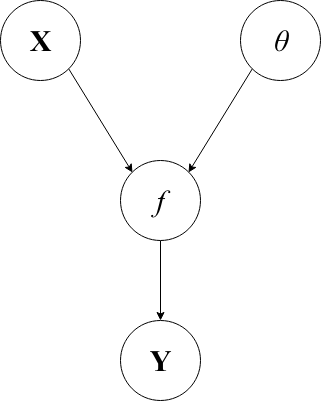
\includegraphics[width=0.5\linewidth]{question_10.png}}
\caption{Graphical model of the joint distribution.}
\label{fig:q10}
\end{figure}

The assumptions that have been made are:

\begin{itemize}
\item $f$ depends on $\bm{\theta}$ and $\mathbf{X}$;
\item $\mathbf{X}$ and $\bm{\theta}$ do not depend on anything;
\item $\mathbf{Y}$ depends on $f$, but is is conditionally independent of $\mathbf{X}$ and $\bm{\theta}$.
\end{itemize}

\subsubsection*{Question 11}

The marginalisation $p(\mathbf{Y|X,\bm{\theta}})$ connects the prior and the data because we now have a way to directly generate $\mathbf{Y}$ values given $\mathbf{X}$ and $\bm{\theta}$ values without knowing the actual form of $f$.
\par
Because we are uncertain about $f$, when we marginalise it out, the uncertainty gets pushed onto $\mathbf{Y}$.
\par
The fact that $\bm{\theta}$ is left on the left hand side of the expression after marginalisation means that it is needed, along with $\mathbf{X}$, to calculate $\mathbf{Y}$. This implies that $\mathbf{Y}$ is dependent on theta.

\begin{figure}[htbp]
\centerline{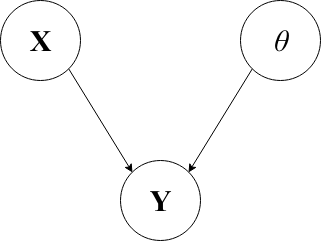
\includegraphics[width=0.5\linewidth]{question_11.png}}
\caption{Graphical model of the marginalised distribution.}
\label{fig:q11}
\end{figure}

The graphical model of the marginal $p(\mathbf{Y|X},\bm{\theta})$ is shown in Figure \ref{fig:q11} and shows how $\mathbf{Y}$ is now dependent on only $\mathbf{X}$ and $\bm{\theta}$.  The function $f$ (and its uncertainty) has been "baked in" to $\mathbf{Y}$.

%Use the model diagram to help?
%Marginalisation is the average of some distributions
%It is a weighted average of some functions, based on how likely each function is
\subsection{Practical}
\subsubsection{Linear Regression}
\subsubsection*{Question 12.1}

The prior distribution over $\mathbf{W}$ can be seen in the middle column of the top row of Figure \ref{fig:q12}. The red cross represents the true value of $\mathbf{W}$. The spherical covariance gives rise to a symmetrical distribution.

The rightmost column of the top row of Figure \ref{fig:q12} shows six random samples drawn from the prior which clearly do not have any well defined direction, which is exactly as expected since we have no data to make predictions with.

\subsubsection*{Question 12.2}

The second row of Figure \ref{fig:q12} show the result of picking a single data point. The leftmost column plots the likelihood distribution in $\mathbf{W}$-space of the data point. The middle column shows the posterior distribution after the likelihood has been combined with the prior. It can be seen visually that the prior has been squashed along the dimension of the likelihood. 

\subsubsection*{Question 12.3}

The rightmost column shows that the sampled functions now all pass through the observed data point, but do not yet agree completely in direction.

\subsubsection*{Question 12.4}

The lower two columns of Figure \ref{fig:q12} show the likelihood, posterior and data space samples after adding two and twenty points respectively. 

\begin{figure}[htb]
\centerline{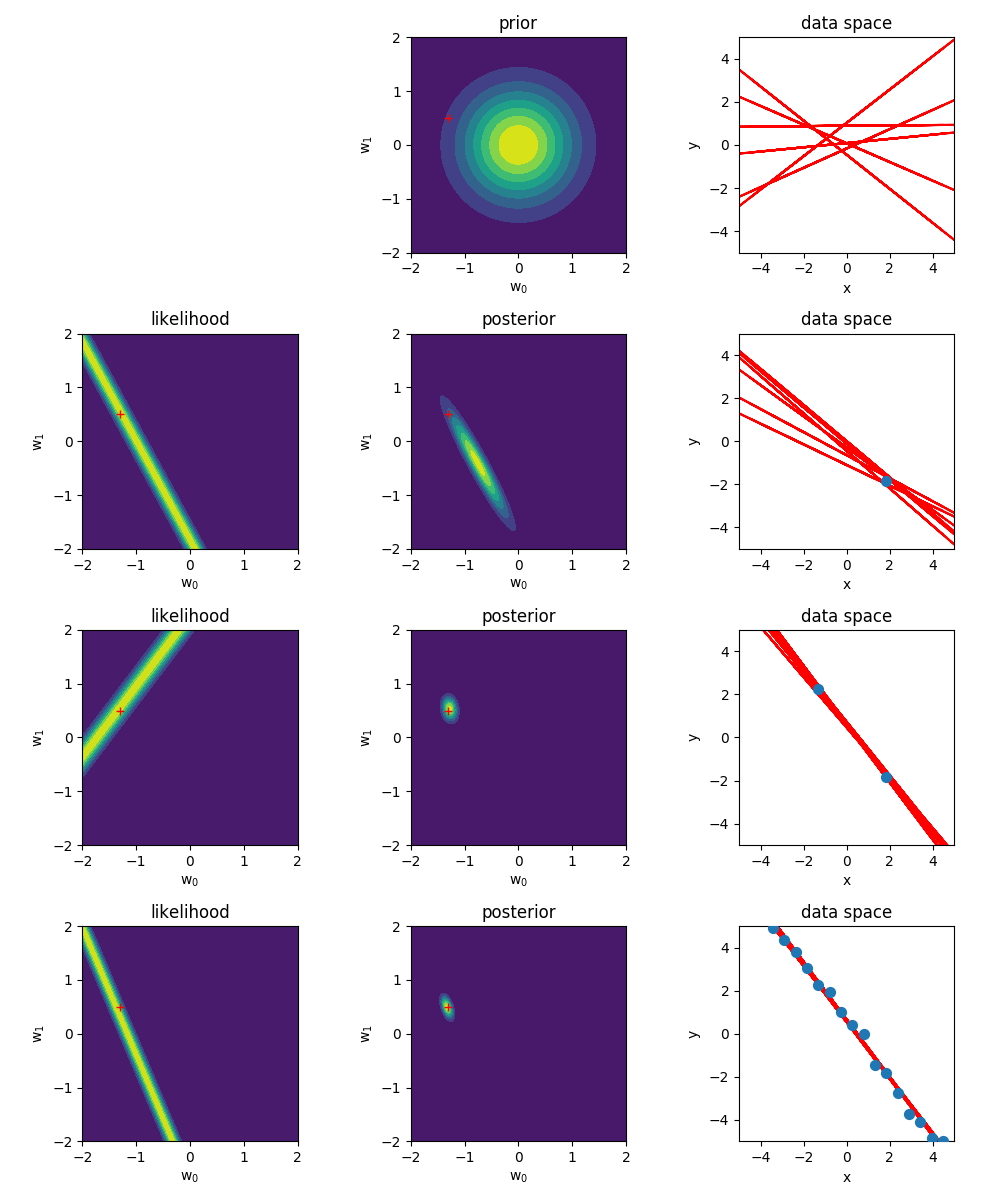
\includegraphics[width=\linewidth]{q12.png}}
\caption{Implementation of linear regression. The left hand column plots the likelihood. The middle column plots the prior/posterior, and the right hand column shows six random sample functions. Plots are drawn after one, two and twenty data points are revealed.}
\label{fig:q12}
\end{figure}

\subsubsection*{Question 12.5}
After a single data point is added, we can see that the posterior distribution begins to squash in one direction to converge onto the parameters $\mathbf{W}$. When we sample from this distribution, there are many lines passing through the point at different gradients, which is because we cannot define two parameters from a single data point. As we begin to reveal more data, the posterior distribution centres onto $\mathbf{W}$ and the sample functions fit more closely to the data points. This is exactly what we want to happen as it shows that we have relearned the parameters of the model used to generate the data $\mathbf{X}$.

\subsubsection*{Question 12.6}
The posterior converges on the position of $\mathbf{W}$ because after a new data point is added, we update the parameters using the newly calculated mean and covariance. As we see more data, we become more and more confident about the true value of $\mathbf{W}$.


\subsubsection{Non-parametric Regression}
\subsubsection*{Question 13}

Figure \ref{fig:q13} shows three examples of samples taken from a GP prior with a squared exponential covariance function that has a single hyper-parameter $l$, which encodes the length scale of the sample functions. The three values of $l$ are 0.1 (a), 0.5 (b) and 5 (c).

\begin{figure}[htb]
\centering
\begin{subfigure}{.5\linewidth}
  \centering
  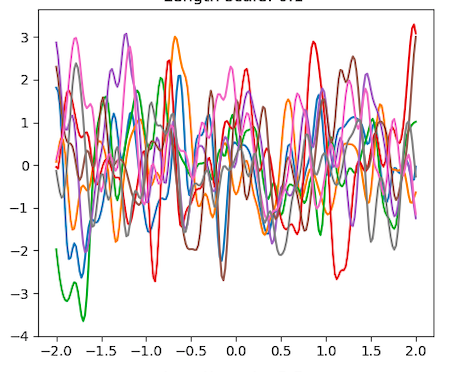
\includegraphics[width=.9\linewidth]{ls01.png}
  \caption{lengthscale of 0.1.}
  \label{fig:sub1}
\end{subfigure}%
\begin{subfigure}{.5\linewidth}
  \centering
  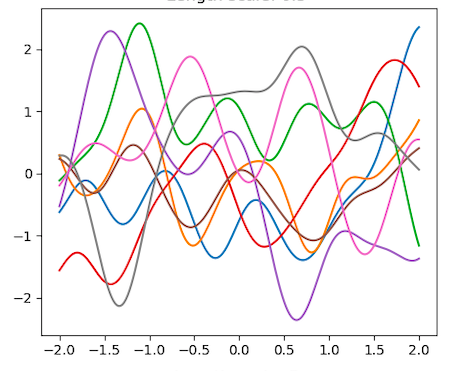
\includegraphics[width=.9\linewidth]{ls05.png}
  \caption{lengthscale of 0.5.}
  \label{fig:sub2}
\end{subfigure}
\begin{subfigure}{.5\linewidth}
\centering
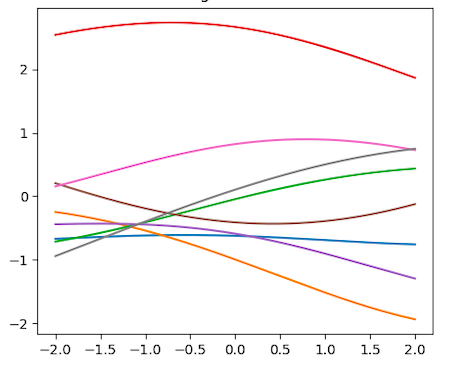
\includegraphics[width=0.9\linewidth]{ls5.png}
\caption{lengthscale of 5}
\end{subfigure}
\caption{Squared exponential with varying length scales. }
\label{fig:q13}
\end{figure}

Increasing the lengthscale of the covariance function allows us to constrain the smoothness of the sample functions. A smaller lengthscale creates functions with more rapid changes than those with a larger lengthscale. This is because a higher lengthscale means that, for two random variables $x_i$ and $x_j$ where the covariance is $k(x_i, x_j)$, their instantiations as $f_i$ and $f_j$ are similar. 

Choosing a larger lengthscale encodes the assumption that a smoother function with lower frequency is preferable to high frequency, more oscillatory functions. In other words, we prefer functions that change less rapidly.

\subsubsection{Question 14}

The predictive posterior distribution is a Gaussian given by 

\begin{align}
  p(\mathbf{Y}_{N+1}|\mathbf{Y}) = \mathcal{N}(\mathbf{M}_{N+1}, \mathbf{C}_{N+1})
\end{align}

where

\begin{equation}
  \mathbf{M}_{N+1} = \mathbf{k^T}\mathbf{C}_N^{-1}\mathbf{Y} \\
  \mathbf{C}_{N+1} = c - \mathbf{k^T}\mathbf{C}_N^{-1}\mathbf{k} 
\end{equation}

and $\mathbf{C_N}$ is the previous covariance matrix, $\mathbf{k}$ has elements $k(\mathbf{x}_n, \mathbf{x}_{N+1}$ (i.e. the kernel function invoked with all the previous data points and the new data point) and $c$ is a scalar that equals $k(\mathbf{x}_{N+1}, \mathbf{x}_{N+1}$ (i.e. the kernel function over just the new data point).

Figure \ref{fig:q14} shows three rows of the process of computing the predictive posterior and sampling from it for the three different length scales. The first column is the random samples from the prior. The middle column shows the noisy data points and the generated predictive mean, with the true function plotted underneath. It also shows the predictive variance, shaded in blue. The last column shows samples from the predictive posterior.

It is clear from the plots that the samples from the posterior are more or less following the observed data. Using a longer length scale results in functions that more closely resemble the true function. If the length scale is too short, it is almost as if the functions have too many degrees of freedom and oscillate up and down quite a lot in order to pass as close as possible to the observed data points. This is not necessarily desirable as it suggests that overfitting may be occurring.

The functions do not pass through the data points exactly, due to the additive noise. Setting $\sigma$ to zero gets rid of this residual noise and causes the functions to go exactly through the data. However, this causes the functions to oscillate more rapidly as if they are being ``forced" to pass through exact points.

\begin{figure}[!htb]
\centerline{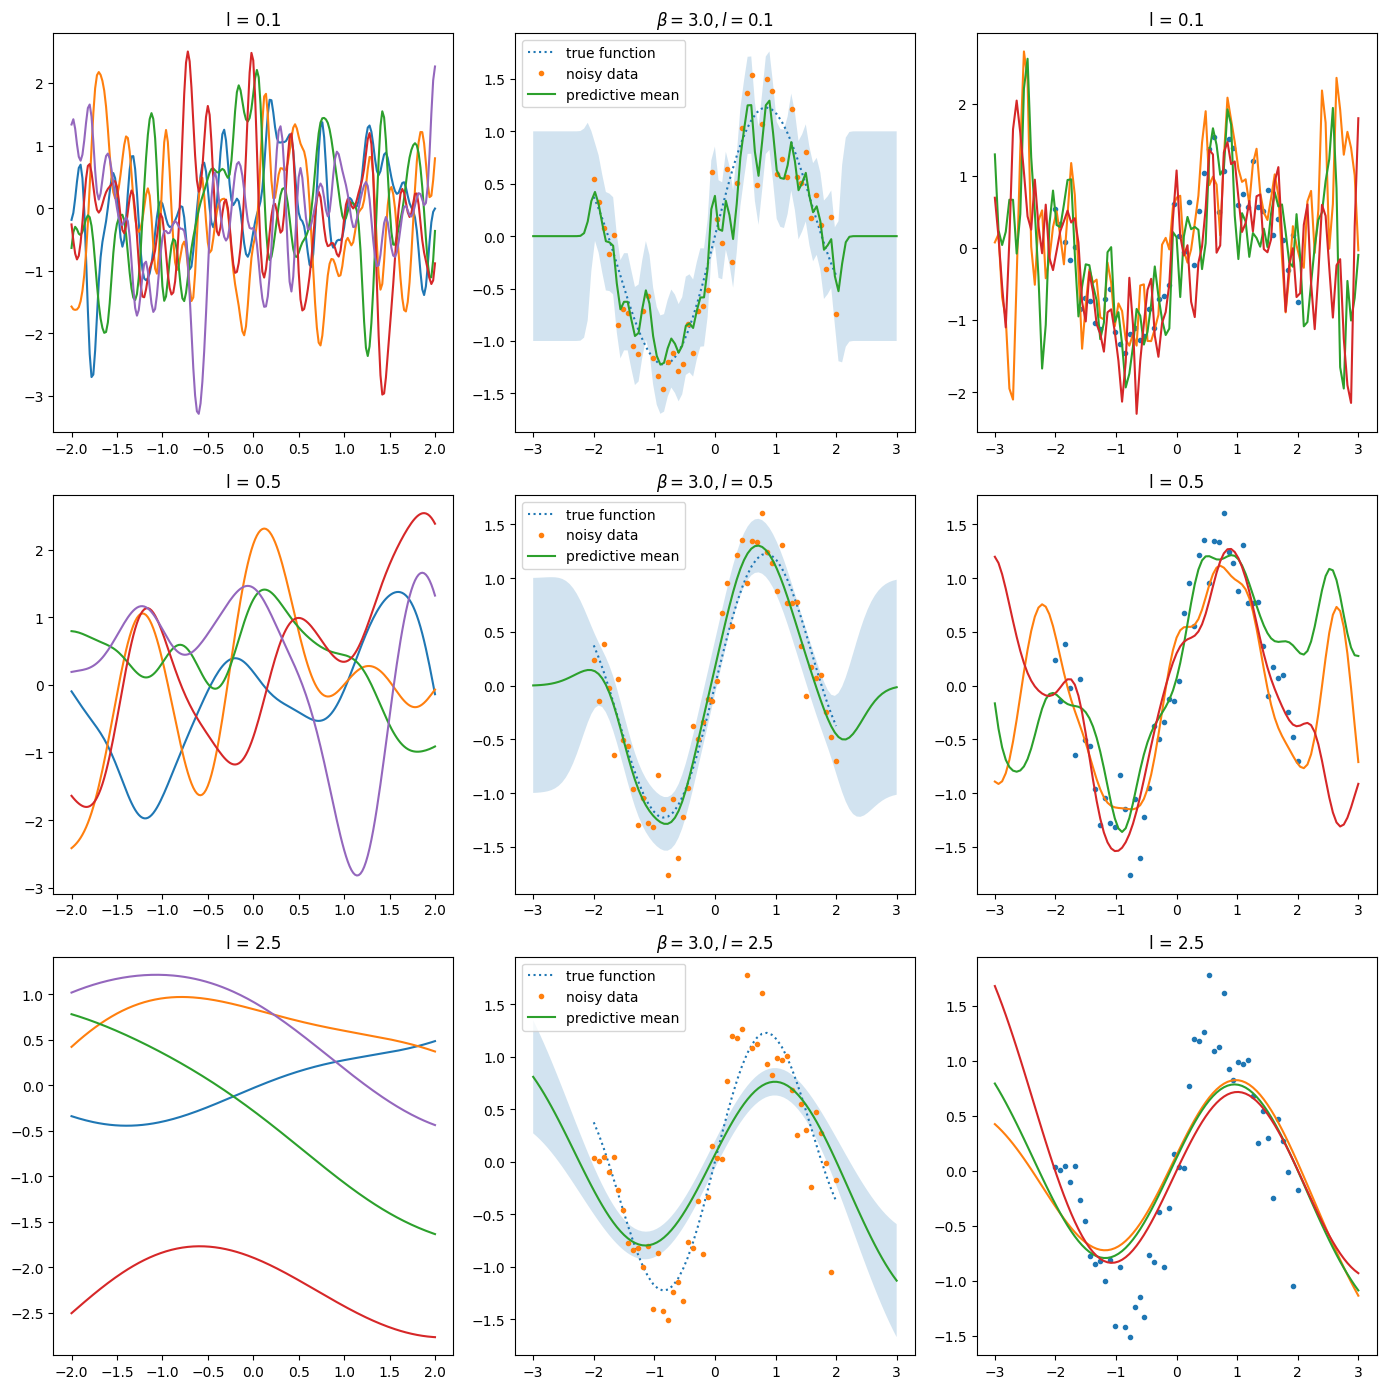
\includegraphics[width=\linewidth]{non_parametric_regression.png}}
\caption{Implementation of non-parametric regression with changing lengthscales. }
\label{fig:q14}
\end{figure}

It is interesting to note that the predictive variance ``falls off" more sharply in regions where there is no data when using a shorter length scale. This is because a shorter length scale produces functions that change more rapidly, so we can be less certain about where adjacent functions will intersect. With a longer length scale, the opposite is true; since we can be fairly sure that the function isn't going to change very rapidly we can make a decent estimate as to where it will intersect in adjacent regions.

%functions not passing exactly through the data, do you have a diagonal term?
%If you look at slide 66 in lecture 6, if you set \sigma=0 then the functions
%should go straight through the data, if you have it larger than zero you have
%a "residual" variance that will be like a noise that can never be removed.



\section{Posterior}

\subsubsection*{Question 15}
We use our beliefs in order to find a starting point (or ``handle") for a particular problem. These beliefs allow us to make assumptions about either the input data itself or the relationship between the inputs and the outputs (i.e. the parameters). These assumptions are used to formulate our prior distributions.

In other words, assumptions are what we assume to be true about something. If we had all the data we required for a problem, there would be no need to assume anything. Making assumptions based on beliefs gives us a way to reason about a problem when we have very little information.

A preference is an assumption that we want to use because it is easier to do so. A preference does not necessarily represent some truth about a variable, but is rather used for convenience. For example, using a Gaussian likelihood so that a posterior distribution is also Gaussian, or ``preferring" a certain class of functions over another because it simplifies calculations in some way.

\subsubsection*{Question 16}

Since the covariance matrix is spherical, we have assumed that the latent input variables are independent and that they are centred around the origin. 

\subsubsection*{Question 17}

One way to obtain the marginal distribution $p(\mathbf{Y|W})$ would be to write out the exponents of the likelihood and the prior and do a bunch of algebra to work out the actual integral. But there is a simpler way.

Firstly, we know that $\mathbf{Y = WX + \epsilon}$ and we know that $\mathbf{X}$ is Gaussian since we put a prior over it. We know that we can do any linear transformation to a Gaussian and it is still a Gaussian because Gaussians are closed under linear transformation. So we know that $p(\mathbf{Y|W})$ is going to be a gaussian. All we need to do is work out the mean and the covariance of the distribution we are looking for.

We know that the mean is the expectation of $\mathbf{Y}$, so we can therefore write

\begin{align} \label{eq:6}
  \mathbb{E}[\mathbf{Y}] = \mathbb{E}[\mathbf{WX} + \epsilon].
\end{align}

We know the expected value of $\mathbf{X}$ since we picked a prior over $\mathbf{X}$ and gave it a zero mean, so it will be zero. We can also ignore $\epsilon$ in the expectation since it is just a noise parameter. Therefore we can deduce that the mean $\mu$ is just going to be zero.

Now to work out the covariance, we know that it is going to be the expected value of $\mathbf{Y}$ multiplied by its transpose, which we can write similarly to (\ref{eq:6}) as

\begin{align}
  \mathbb{E}[\mathbf{YY^T}] = \mathbb{E}[\mathbf{(WX + \epsilon)(WX + \epsilon)^T}] \\
  = \mathbb{E}[\mathbf{WXX^TW^T}] + \mathbb{E}[\mathbf{\epsilon\epsilon^T}]
\end{align}

The expectation of the noise parameter $\epsilon$ we have already defined as being $\sigma^2\mathbf{I}$. Since our prior over $\mathbf{X}$ was zero-mean, we know that $\mathbf{XX^T}$ is going to be the identity matrix, therefore can simply write the covariance as

\begin{align}
  \mathbb{E}[\mathbf{Y}] = \mathbf{WW^T + \sigma^2I}
\end{align}

which gives us the resulting marginal distribution

\begin{align}
  p(\mathbf{Y|W}) = \mathcal{N}(0, \mathbf{WW^T + \sigma^2I})
\end{align}

and we are done.

\subsubsection*{Question 18.1}
All three estimation techniques attempt to find some parameters that maximise a distribution. ML simply maximises the likelihood, and does not take any prior information prior into account, which can often be seen as a limitation. MAP attempts to do better by taking the prior into account and maximising on the posterior distribution instead, however that makes it more computationally expensive. ML can be seen as a special case of MAP which assumes a uniform prior of the parameters. Type-II ML maximises the marginal likelihood after integrating out some parameters and is kind of an in-between stage of ML and MAP.

\subsubsection*{Question 18.2}
With only one data point, ML will be less accurate than MAP since it does not take the prior into account. However as more data is seen, the two will begin to converge on one another. 

\subsubsection*{Question 18.3}
The denominator of the posterior distribution has no bearing on the result as it will always be positive, and depends on the parameters $\mathbf{W}$.  Therefore the two expressions are equivalent.

\subsubsection*{Question 19}

The objective function can be written as:

\begin{multline}
  \mathcal{L}(\mathbf{W}) = -log(p(\mathbf{Y}|\mathbf{W}, \bm{\mu}, \bm{\sigma}^2)) \\
  = -\frac{ND}{2}log(2\pi) - \frac{N}{2}log|\mathbf{C}| - tr(\mathbf{(YC)^{-1}Y^T})
\end{multline}

where $\mathbf{C} = \mathbf{WW^T} + \bm{\sigma^2}\mathbf{I}$. The gradients of the objective function with respect to the parameters can be written as:

\begin{multline}
  \frac{\partial \mathcal{L}}{\partial \mathbf{W}} = tr(\mathbf{C^{-1}(WJ_{ij} +  J_{ji}W^T)}) \\
  + tr(\mathbf{Y^TY(-C^{-1}(WJ_{ij} +  J_{ji}W^T)C^{-1}})
\end{multline}

where $\mathbf{WJ_{ij} +  J_{ji}W^T}$ = $\frac{\partial \mathbf{C}}{\partial \mathbf{W_{ij}}}$.

\subsubsection*{Question 20}
$\mathbf{Y}$ is dependent on both $\mathbf{X}$ and $\mathbf{\theta}$, which both contain a level of uncertainty. By marginalising out $f$, the uncertainty will be filtered down into the marginal distribution of $\mathbf{Y}$. 
\par
Marginalising out $f$ is easier than $\mathbf{X}$, as $f$ is only a dependency of $\mathbf{Y}$, whereas $\mathbf{X}$ is a dependency of both $f$ and $\mathbf{Y}$.
Because $\mathbf{X}$ is a dependency of $f$ and $\mathbf{Y}$, we would have to deal with both $f$ and $\mathbf{Y}$ when marginalising it out. 





\subsubsection*{Question 21}

We first mapped the input variables $\mathbf{x}$ non-linearly to a 2D space and plotted the result. This gives a uniform spiral shape as seen in Figure \ref{fig:sub1}. We then mapped this linearly to a 10D space. Given the objective function and gradients from above, we then minimised the log likelihood to "learn" the linear mapping parameters W. Using the new parameters, we performed the reverse of the linear mapping back to 2D space and obtained another (slightly different) spiral, a particular example of which can be seen in Figure \ref{fig:q21b}.

\begin{figure}[!htb]
\centering
\begin{subfigure}{.5\linewidth}
  \centering
  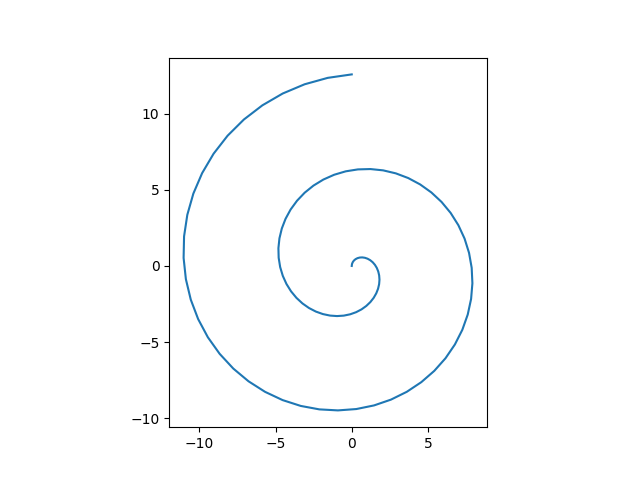
\includegraphics[width=.9\linewidth]{q21_a.png}
  \caption{Original 2D subspace.}
  \label{fig:q21a}
\end{subfigure}%
\begin{subfigure}{.5\linewidth}
  \centering
  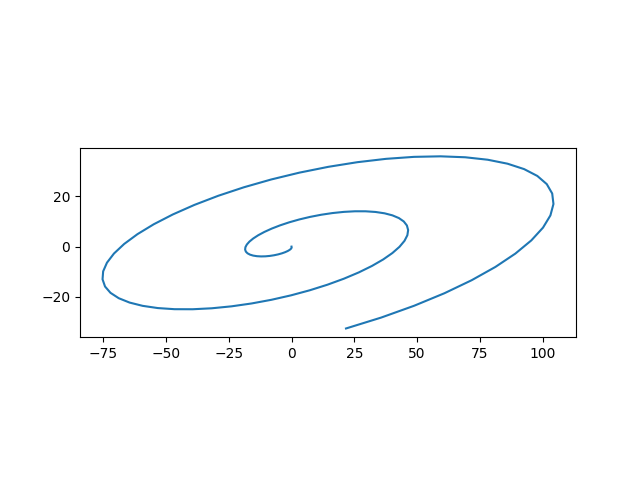
\includegraphics[width=.9\linewidth]{q21_b.png}
  \caption{Subspace learnt via Type-II ML.}
  \label{fig:q21b}
\end{subfigure}
\begin{subfigure}{.5\linewidth}
  \centering
  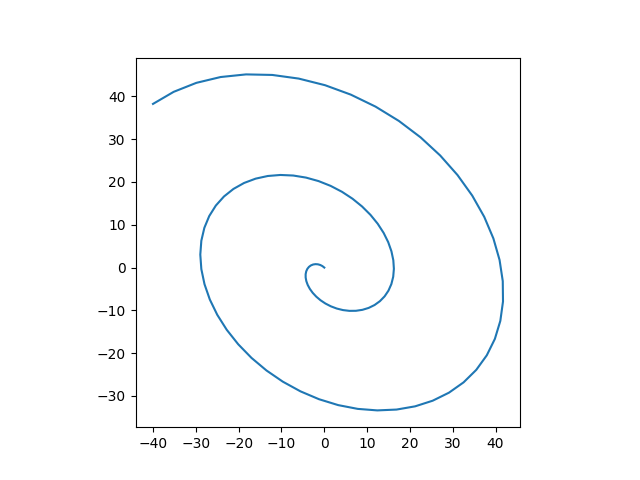
\includegraphics[width=.9\linewidth]{q22.png}
  \caption{Random subspace.}
  \label{fig:q22}
\end{subfigure}
\caption{Subspaces representing a 2D non-linear mapping from a 1D input vector. }
\end{figure}

We expected the recovered shape to be more similar to the original shape. We considered that there may be an error in the minimisation process (probably somewhere in computing the gradients). We obtain a different shape every time we run the code, due to the randomised starting point for the gradient descent. We assume this is because there are many local minima in the 10D space, and the gradient descent is not guaranteed to find the global minima and is likely to get stuck in a local minima.

Since we have only learned the parameters for the linear part of the mapping and not the non-linear part, it does not immediately appear possible to recover the original latent variables themselves.

\subsubsection*{Question 22}

Choosing any randomly initialised W matrix and performing the reverse mapping also results in a spiral shape, as can be seen in Figure \ref{fig:q22}. However, the shape is slightly different in dimension. In fact, this shape is often more similar to the original than the one obtained via gradient descent. It is not understood why this is the case.

\section{The Evidence}

\subsubsection*{Question 23}

$\mathcal{M}_0$ can be thought of as the simplest possible model because it just assigns the exact same probability for all possible data sets and it has no parameters whatsoever. However, it can also be considered the most complex model for the same reason, in that it can make predictions for all data sets i.e. it predicts that data will be drawn from a large range of possibilities. Other models that concentrate their probability masses around a limited number of data sets can be considered simpler than $\mathcal{M}_0$.

This begs the question of what the definition of complexity is - it could be argued that the number of parameters has no bearing on the complexity of the model at all, and that we need some other measure of complexity (such as the spread of probability mass).

\subsubsection*{Question 24}

The more parameters a model has the more degrees of freedom it can use to segment the data space. The single parameter model $\mathcal{M}_1$ is best suited to model data sets where there is a simple linear segmentation of the two regions of the data space (i.e. conceptually drawing a line where all the X's are on one side and all the O's on the other). However, there are only a few data sets that can be segmented in this way, so we would expect it to be less flexible than models with more parameters. $\mathcal{M}_2$ and $\mathcal{M_3}$ should have more flexibility to draw boundaries in the data space to segment different types of region, so will me more likely for a larger range of data sets. However, there are some data sets for which none of the parameterised models will be able to capture, in which case $\mathcal{M}_0$ will end up being the most likely.

\subsubsection*{Question 25}

By choosing a prior with a large variance, we are spreading the probability mass across a large portion of the parameter space i.e. choosing a wide distribution. The value of the mean should not matter in this case, as the distribution should be invariant under translation.

\subsubsection*{Question 26}

The sum of the evidence for each model for the whole of $\mathcal{D}$ sums to one (allowing for some numerical error tolerance). This is has to be the case since each expectation is a probability distribution and therefore by definition must sum to one.

\subsubsection*{Question 27}

Figure \ref{fig:q27} shows the plots of the evidence over $\mathcal{D}$ for each of the four models. The evidence distribution for $\mathcal{M}_1$ is the most obvious, since it simply assigns equal probability to each data point and is therefore a simple flat line where the probability mass is distributed equally for all $\mathcal{D}$. The rest of the models appear to generally distribute their probability masses in relation to the number of their parameters, with the most complex (most parameters) model having the widest and shallowest distribution and the least complex (fewest parameters) having the tallest and narrowest distribution. This makes sense since these models are able to segment the data space in more flexible ways.

\begin{figure}[htb]
\centerline{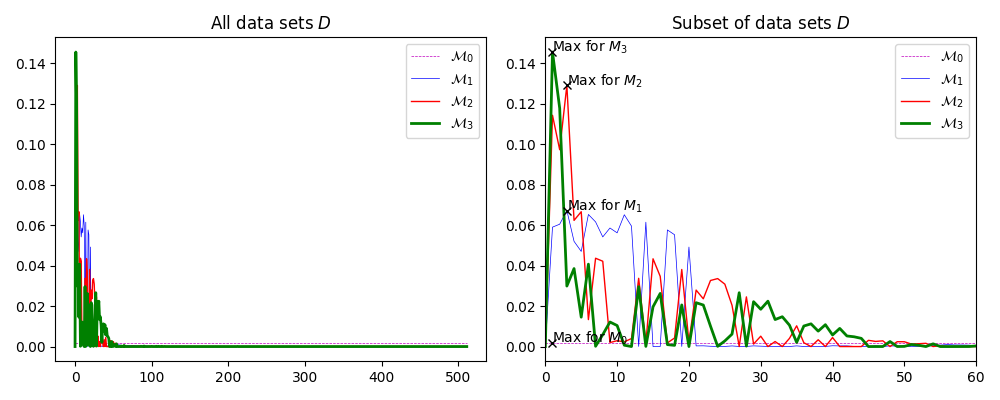
\includegraphics[width=\linewidth]{q27.png}}
\caption{Evidence distributions for the four models. The most likely data set for each model is annotated with a cross.}
\label{fig:q27}
\end{figure}

\subsubsection*{Question 28}

Figure \ref{fig:q28} shows the most likely and least likely data sets for each model. The first two data sets are for $\mathcal{M_0}$ which happen to be the same - in fact by definition all data sets are equally likely with this model so these are just the first items in the array.

\begin{figure}[htb]
\centerline{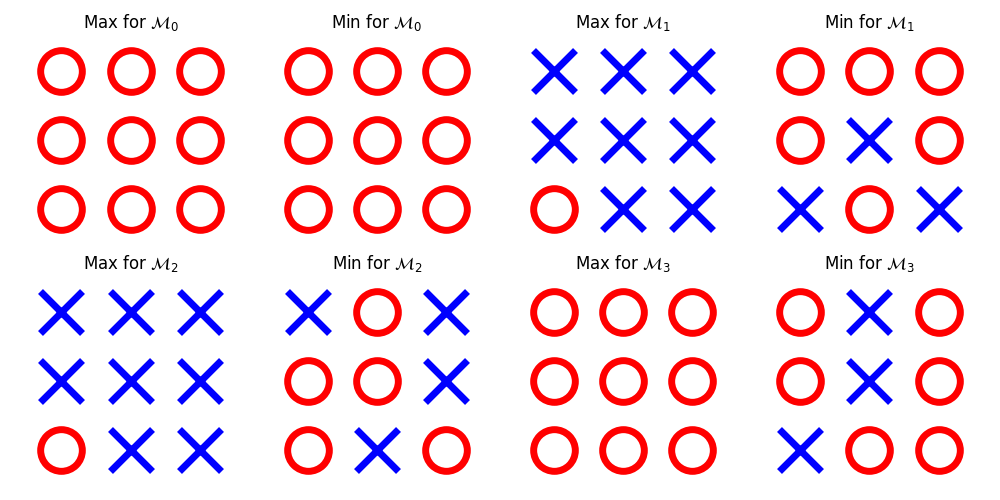
\includegraphics[width=\linewidth]{q28.png}}
\caption{Most likely (max) and least likely (min) data sets for each model.}
\label{fig:q28}
\end{figure}

The least likely data sets for $\mathcal{M}_1$, $\mathcal{M}_2$ and $\mathcal{M}_3$ make sense since they are all have complex regions that cannot be segmented linearly therefore none of the models will have enough flexibility to express these. The most likely data set for $\mathcal{M}_3$ makes sense due to its bias term. We would also expect the opposite grid (all X's) to also be equally likely. The most likely data sets for $\mathcal{M}_1$ and $\mathcal{M}_2$ also seem easy to explain using the linear separability argument. 

\subsubsection*{Question 29}

Figure \ref{fig:q29_a} shows the result of changing the covariance matrix of the prior to use a randomly initialised matrix. It appears to have the effect of stretching out the distribution. It does not appear to make much sense to use a non-diagonal covariance matrix in this case, since that would imply some kind of correlation between data sets when clearly there is none.

\begin{figure}[htb]
\centerline{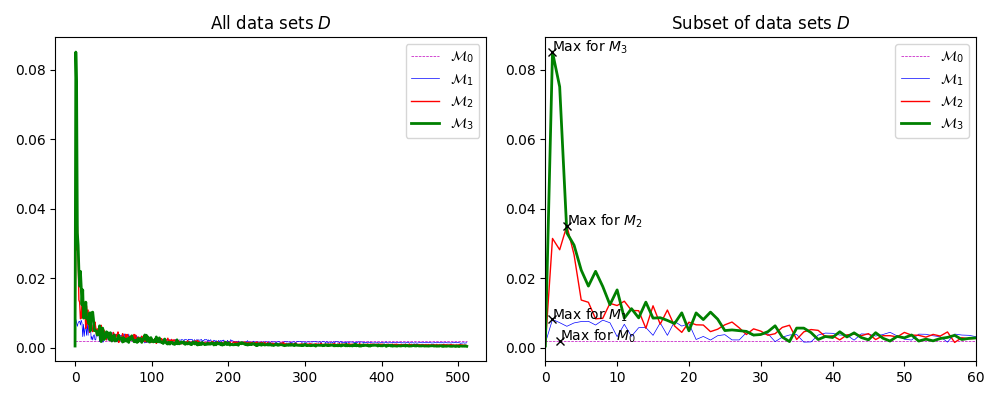
\includegraphics[width=\linewidth]{q29_a.png}}
\caption{Evidence distributions for the four models using a non-diagonal covariance matrix.}
\label{fig:q29_a}
\end{figure}

Figure \ref{fig:q29_b} shows the result of using a non-zero mean. This results in a different plot due to the randomness in the Monte Carlo sampling process, but the actual characteristics of the distributions are similar. This is as expected since shifting the mean of a distribution is an invariant operation.

\begin{figure}[htb]
\centerline{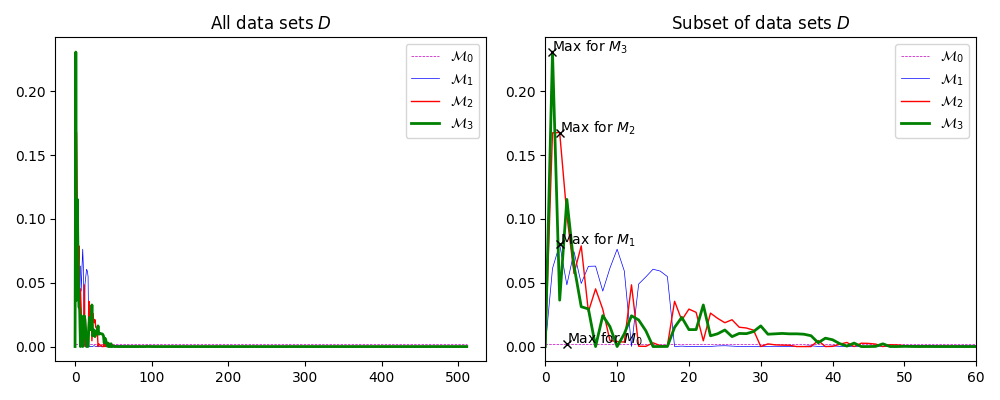
\includegraphics[width=\linewidth]{q29_b.png}}
\caption{Evidence distributions for the four models using a non-zero mean.}
\label{fig:q29_b}
\end{figure}

\section{Final Thoughts}
\subsubsection*{Question 30}
The authors feel that the purpose of this assignment was to introduce the basics of machine learning using a statistical, low level, brutal, sadistic, trauma-inducing and slightly evil approach that is terrifying for those without a strong background in mathematics. Students are thrown in to the deep end of a swimming pool and forced to learn the theory behind the techniques in gory detail before being able to truly understand or implement them. However, in the end, the differences between the various techniques we have explored have started to become clearer (although knowing which technique to pick in which situation based on real data still seems a long way off). One main learning point that is more or less clear is that all the techniques involve making some assumptions about some data, formulating those assumptions into prior distributions and then churning the Bayesian handle to produce some intelligible posterior result.

%----------------------------------------------------------------------------------------
%	BIBLIOGRAPHY
%----------------------------------------------------------------------------------------

\printbibliography[title={Bibliography}] % Print the bibliography, section title in curly brackets

%----------------------------------------------------------------------------------------

\end{document}
